%\documentclass[letter,mathserif,usenames,dvipsnames,aspectratio=169]{gkibeamer}
\documentclass[letter,mathserif,usenames,dvipsnames]{gkibeamer}

%% note: use this for handout mode!
%\documentclass[mathserif,handout,4-on-1]{gkibeamer}


%% note: use this for handout mode!
%%\documentclass[mathserif,handout,4-on-1]{gkibeamer}

\usepackage{amsmath,amssymb,amsthm}
\usepackage{nicefrac}
\usepackage{array}
\usepackage{xspace}
\usepackage{multirow}
%\usepackage{realboxes}
%\usepackage{algorithmic}

\usepackage{graphicx}
\usepackage{booktabs}
\usepackage{enumerate}
\usepackage[absolute,overlay]{textpos}

\usepackage{tikz}
\usetikzlibrary{shapes,positioning,calc,intersections}
\usetikzlibrary{tikzmark,fit,shapes.geometric}
\newcommand{\TargetVariable}[1]{\underline{#1}}
%\usetikzlibrary{arrows,petri,automata,snakes}

\tikzstyle{every transition}=[minimum size=4mm]
\tikzstyle{every place}=[minimum size=4mm]
\tikzstyle{pnplace}=[shape=circle,place,thick,inner sep=0.05mm]
\tikzstyle{pntrans}=[transition,thick,inner sep=0.5mm]

\pgfmathsetseed{\pdfuniformdeviate 10000000} % new seed at each compilation

\usepackage{framedboxes}

\definecolor{lightskyblue}{cmyk}{0.31,0.11,0.0,0.0}
\newcommand{\hilite}{\textcolor{structure}}

\newcommand{\Omit}[1]{}
\newcommand{\NoOmit}[1]{#1}
\newcommand{\tup}[1]{\langle #1 \rangle}
\newcommand{\denselist}{\itemsep 0pt \topsep 0pt}
\newcommand{\sci}[2]{#1\textsc{e}#2}

\newcommand{\TBD}[1]{\textbf{TBD:} #1}

\newcommand{\red}[1]{\textcolor{Red}{#1}}
\newcommand{\green}[1]{\textcolor{OliveGreen}{#1}}

%\usepackage[table]{xcolor}
\usepackage{colortbl}
\newcommand{\G}{\cellcolor[gray]{0.75}}

\renewcommand{\P}{\mathbb{P}}
\newcommand{\R}{\mathcal{R}}


\usepackage{relsize}
\newcommand{\join}{\mathlarger{\Join}}
\DeclareMathOperator{\bigjoin}{\mathlarger{\mathlarger{\mathlarger{\Join}}}}

%% Set bold frame titles
\setbeamerfont{frametitle}{series=\bfseries\centering}

%% This makes invisible the covered items
\setbeamercovered{transparent}

%% This makes the text in second-/third-level lists same font size as
%% in first-level lists
\setbeamerfont{itemize/enumerate subbody}{size=\normalsize}
\setbeamerfont{itemize/enumerate subsubbody}{size=\normalsize}
\setbeamerfont{itemize/enumerate subitem projected}{size=\normalsize}
\setbeamerfont{itemize/enumerate subsubitem projected}{size=\normalsize}

%% This makes the bullets in second/third level list same size as
%% in first-level lists
\makeatletter
%\setbeamertemplate{itemize subitem}{\beamer@usesphere{subitem projected}{bigsphere}}
%\setbeamertemplate{itemize subsubitem}{\beamer@usesphere{subsubitem projected}{bigsphere}}
\setbeamertemplate{itemize subitem}{\tiny\raise1.5pt\hbox{\donotcoloroutermaths$\blacktriangleright$}}
%\setbeamercolor{itemize item}{fg=OliveGreen}
%\setbeamercolor{enumerate item}{fg=OliveGreen}
\setbeamercolor{itemize item}{fg=black}
\setbeamercolor{enumerate item}{fg=black}
%\setbeamercolor{itemize subitem}{fg=OliveGreen}
%\setbeamercolor{itemize subsubitem}{fg=default}
\makeatother

%% Reduces list indentation and label space
\setlength{\leftmargini}{1em}
\setlength{\leftmarginii}{0.75em}
\setlength{\leftmarginiii}{0.75em}
\setlength{\labelsep}{.5em}
\setlength{\labelwidth}{1em}

\setbeamersize{text margin left=0.75cm, text margin right=0.75cm}

%% this changes the margins on the hand-out version (I think it is
%% to make it more similar to the slides version).
\mode<handout>{%
  \setbeamersize{text margin left=0.75cm}
  \setbeamersize{text margin right=1.75cm}
}

\newcommand{\naturals}{\ensuremath{\mathbb{N}}}
\newcommand{\reals}{\ensuremath{\mathbb{R}}}
\newcommand{\indicator}[1]{[\![#1]\!]}

\newcommand<>{\textblue}[1]{{\color#2{blue}#1}}
\newcommand<>{\textbg}[1]{{\color#2{bg}#1}}

\newcommand<>{\gray}[1]{\textcolor#2{gray}{#1}}
\newenvironment<>{grayenv}{\color#1{gray}}{}

%\newcommand{\Alert}[1]{\alert{\bf #1}}
\newcommand{\Alert}[1]{\textcolor{blue!70!black}{\bf #1}}
\newcommand{\AlertSecondary}[1]{\textcolor{blue!70!black}{#1}}
\newcommand{\RedAlert}[1]{\textcolor{red}{\bf #1}}

\definecolor{customblue}{rgb}{0.129216,0.188235,0.709804}


%\setbeamertemplate{blocks}[framed]
%\setbeamercolor{block title}{fg=darkblue!80!yellow, bg=gray!30}%white!80!yellow!85!orange}
%\setbeamercolor{block title}{fg=black, bg=gray!40}%white!80!yellow!85!orange}
%\setbeamercolor{block body}{fg=darkblue!80!yellow, bg=gray!20}%yellow!20!orange}
%\setbeamercolor{block body}{fg=black, bg=gray!20}%yellow!20!orange}
\setbeamerfont{block title}{series=\bfseries}
\setbeamerfont{block body}{series=\itshape}
\setbeamercolor{block title}{fg=white, bg=customblue!100}
\setbeamercolor{block body}{fg=black, bg=customblue!5}
\setbeamercolor{postit}{bg=yellow!50!white}


\newcommand{\SAS}{\ensuremath{\text{SAS}^+}\xspace}
\newcommand{\hplus}{\ensuremath{h^+}\xspace}
\newcommand{\hlmcut}{\ensuremath{h^{\text{LM-cut}}}\xspace}
\newcommand{\myhlmcut}{\ensuremath{h^{\text{LM-cut}}_{\text{ours}}}\xspace}
\newcommand{\hla}{\ensuremath{h^{\text{LA}}}\xspace}
\newcommand{\hms}{\ensuremath{h^{\text{M\&S}}}\xspace}
\newcommand{\HSPf}{\ensuremath{\text{HSP}^*_F}\xspace}
\newcommand{\hseq}{\ensuremath{h^{\text{SEQ}}}\xspace}
\newcommand{\hiseq}{\ensuremath{h^{\text{iSEQ}}}\xspace}
\newcommand{\hseqsafe}{\ensuremath{h^{\text{SEQ}}_\text{safe}}\xspace}
\newcommand{\hm}{\ensuremath{h^m}\xspace}

\newcommand{\pit}[1]{\text{pit@$#1$}}
\newcommand{\breeze}[1]{\text{breeze@$#1$}}
\newcommand{\map}[1]{\text{cell@$#1$}}
\newcommand{\sensor}[1]{\text{sensed@$#1$}}

\newcommand{\ellipse}[4]{
  \visible<#1>{
  \begin{tikzpicture}[remember picture,overlay]
  \coordinate[draw,line width=.75pt,blue!70!black,ellipse,inner xsep=#2, inner ysep=#3,fit={(pic cs:#4)}] {};
  \end{tikzpicture}
  }
}

\newcommand{\mymark}[1]{\raisebox{3pt}{\tikzmark{#1}}}

\newcommand{\widthofbold}[1]{%
\settowidth{\dimen0}{\textbf{#1}}%
\makebox[\dimen0]{#1}}
\newcommand<>{\bold}[1]{%
\alt#2{\textbf{#1}}{\widthofbold{#1}}}
\makeatother

\mode<beamer>{
  \title{\bf Algoritmos para Juegos con Informaci\'on\\Incompleta y No Determinismo}
  \author{Rubmary Rojas}
  \institute{Universidad Sim\'on Bol\'{\i}var, Caracas, Venezuela}
  \date{Enero 2020}
}

% Only if sectionpage is undefined
%\newcommand{\sectionpage}{}

\definecolor{c231f20}{RGB}{35,31,32}
\newcommand{\logousb}[1][0.0333]{%
\begin{tikzpicture}[y=0.80pt,x=0.80pt,yscale=-1, inner sep=0pt, outer sep=0pt]
\begin{scope}[cm={{1.25,0.0,0.0,-1.25,(0.0,142.5)}}]
  \begin{scope}[scale=#1]
    \path[fill=c231f20,even odd rule] (852.7580,526.1290) -- (779.6020,496.6410) --
      (777.0080,504.4880) -- (556.5040,415.5860) .. controls (550.8120,413.5230) and
      (547.0160,408.1170) .. (547.0160,402.0700) -- (547.0160,53.4688) --
      (555.6760,48.5000) -- (555.6760,3.0898) -- (497.4920,3.0391) --
      (497.4920,75.9414) -- (504.9220,73.9492) -- (504.9220,401.8010) .. controls
      (504.9220,427.0270) and (521.9060,449.1090) .. (546.3120,455.6370) --
      (763.9840,543.8480) -- (761.1170,552.5000) -- (852.7580,589.4410) --
      (944.6330,551.4100) -- (941.8320,543.0000) -- (1158.5000,454.2230) .. controls
      (1181.5200,446.1020) and (1200.6000,432.7580) .. (1200.6000,400.5550) --
      (1199.3600,68.9453) -- (1206.8300,72.3359) -- (1206.8300,0.6445) --
      (1148.6400,0.6445) -- (1148.6400,45.2930) -- (1157.3200,49.6680) --
      (1158.5000,402.0510) .. controls (1158.5000,408.1050) and (1151.7200,413.3090)
      .. (1146.0300,415.3710) -- (928.5080,504.4690) -- (925.9140,496.6250) --
      (852.7580,526.1290);
    \path[fill=c231f20,even odd rule] (852.7580,414.3950) -- (811.9140,397.9800) --
      (809.1840,407.2420) -- (648.5160,342.4650) -- (648.5160,19.2695) --
      (657.1760,15.2930) -- (657.1760,2.9414) -- (599.0000,3.1367) --
      (599.0000,31.5977) -- (606.4260,31.4023) -- (606.4260,370.9570) --
      (795.9100,447.3590) -- (793.1990,455.5470) -- (852.7580,479.5040) --
      (912.2070,454.0470) -- (909.7230,446.5980) -- (1097.8500,368.4490) --
      (1097.8500,29.8320) -- (1104.0000,29.0625) -- (1104.0000,0.6445) --
      (1045.8500,0.6445) -- (1045.8500,13.9688) -- (1055.7600,18.5898) --
      (1055.7600,340.6520) -- (896.3550,406.4530) -- (893.5080,397.9060) --
      (852.7580,414.3950);
    \path[fill=c231f20,even odd rule] (852.7580,697.0160) -- (729.7110,647.4180) --
      (732.2030,639.8750) -- (493.0780,543.4410) .. controls (438.4020,517.9960) and
      (403.4260,463.1990) .. (403.4260,402.9800) -- (403.4260,136.7810) --
      (395.9880,141.3520) -- (395.9880,9.6445) .. controls (415.2380,6.7813) and
      (434.8750,5.0391) .. (454.2380,4.5938) -- (454.1800,102.7770) --
      (444.2770,109.7420) -- (444.2770,406.9840) .. controls (444.2770,407.0390) and
      (444.2770,407.0940) .. (444.2770,407.1410) .. controls (444.2770,448.5430) and
      (468.3200,486.2110) .. (505.9100,503.7030) -- (745.0390,601.0980) --
      (748.0080,592.1290) -- (852.7580,634.3670) -- (957.9880,591.5040) --
      (961.0900,600.8160) -- (1199.3600,502.6600) .. controls (1235.5100,482.3050)
      and (1258.9500,449.6520) .. (1261.2400,407.1090) .. controls
      (1261.2500,407.0590) and (1261.2400,407.0040) .. (1261.2400,406.9530) --
      (1259.6700,105.1250) -- (1250.1800,97.8828) -- (1249.4200,0.6445) .. controls
      (1268.7800,1.0937) and (1288.8500,3.0312) .. (1308.1000,5.8945) --
      (1308.5300,136.1720) -- (1302.1000,133.0310) -- (1303.1000,409.4060) ..
      controls (1302.1000,464.4800) and (1265.9600,516.8090) .. (1212.7200,541.9730)
      -- (974.1290,638.5940) -- (976.5200,647.1480) -- (852.7580,697.0160);
    \path[fill=c231f20,even odd rule] (892.3670,0.6445) -- (892.3670,232.3200) --
      (852.7580,249.5900) -- (811.9140,233.1250) -- (811.9140,0.6445) --
      (892.3670,0.6445);
    \path[fill=c231f20,even odd rule] (852.7580,315.7420) -- (953.0230,273.8870) --
      (953.0230,0.6445) -- (993.8710,0.6445) -- (993.8710,301.2850) --
      (878.3870,348.4920) -- (878.5860,358.0000) -- (852.7580,368.4880) --
      (824.8750,357.2460) -- (826.8710,348.7540) -- (710.4100,301.7930) --
      (710.4100,0.6445) -- (750.0270,0.6445) -- (750.0270,274.3200) --
      (852.7580,315.7420);
    \path[fill=c231f20,even odd rule] (852.7580,742.9650) -- (716.2970,687.9610) --
      (713.5860,696.1410) -- (468.3240,596.7540) .. controls (392.3790,561.4140) and
      (343.8050,485.3090) .. (343.8050,401.6680) -- (343.8050,176.9450) --
      (353.9060,169.5860) -- (353.9180,17.9219) .. controls (333.3830,23.0156) and
      (312.9570,29.5859) .. (293.2580,37.3828) -- (293.2540,209.1560) --
      (301.9180,205.1760) -- (301.9180,399.7460) .. controls (301.9180,506.4300) and
      (366.8360,602.4690) .. (465.9260,642.4530) -- (700.0660,737.0080) --
      (697.5740,744.5430) -- (852.7580,807.1020) -- (1008.6400,743.5860) --
      (1006.1200,736.0230) -- (1245.9500,638.0980) .. controls (1345.0400,595.3320)
      and (1404.8400,506.3980) .. (1404.8400,399.7150) -- (1404.8400,200.3830) --
      (1413.1600,203.3550) -- (1411.0700,33.7734) .. controls (1391.3600,25.9805)
      and (1372.2300,19.2070) .. (1351.7000,14.1211) -- (1352.9000,164.8870) --
      (1361.5200,170.6520) -- (1363.9100,401.6370) .. controls (1359.9200,485.2810)
      and (1312.1400,563.3750) .. (1235.7900,596.3280) -- (992.5270,695.2110) --
      (989.9450,687.4530) -- (852.7580,742.9650);
    \path[fill=c231f20,even odd rule] (852.7580,853.3010) -- (684.0860,785.2930) --
      (681.3440,793.5820) -- (436.9180,693.0080) .. controls (353.9060,656.7150) and
      (252.4100,584.7700) .. (242.5000,398.4730) -- (242.5000,243.5820) --
      (252.4100,236.4960) -- (251.0310,59.4492) .. controls (226.6800,67.7656) and
      (208.3520,80.8984) .. (191.7540,94.7852) -- (191.7540,275.5120) --
      (202.0040,271.2540) -- (201.6760,371.8440) .. controls (201.6410,600.1680) and
      (326.5660,699.0390) .. (444.2770,741.1880) -- (668.4140,832.6640) --
      (665.8050,840.5510) -- (853.4730,916.4570) -- (1040.6800,839.7970) --
      (1038.0800,831.9730) -- (1286.2200,730.5270) .. controls (1358.3900,703.7770)
      and (1492.0000,608.8440) .. (1506.3400,414.5620) -- (1506.4100,266.1170) --
      (1516.2600,269.3010) -- (1513.8100,89.7227) .. controls (1499.7900,79.7656)
      and (1478.6100,63.3203) .. (1454.1300,52.5352) -- (1455.6300,232.4450) --
      (1465.4900,239.8120) -- (1465.4900,412.2230) .. controls (1459.6800,482.1090)
      and (1432.3800,625.0660) .. (1266.0200,694.7620) -- (1025.1500,793.1410) --
      (1022.3300,784.6800) -- (852.7580,853.3010);
    \path[fill=c231f20,even odd rule] (853.9490,961.2930) -- (652.6990,880.1520) --
      (648.5160,888.3710) -- (396.4960,784.6050) .. controls (287.1450,741.4380) and
      (154.4220,611.9100) .. (144.4840,416.4140) -- (143.4730,309.9220) --
      (152.1290,303.2500) -- (149.6800,132.0080) .. controls (120.3090,155.2970) and
      (104.9180,175.3280) .. (90.2500,195.8200) -- (91.4805,343.6640) --
      (100.1480,338.1800) -- (101.7500,410.5740) .. controls (108.6680,640.3670) and
      (253.2770,772.3440) .. (395.9880,830.3910) -- (636.3790,929.4800) --
      (633.7230,937.5040) -- (852.7580,1025.8200) -- (1072.0700,937.2970) --
      (1070.1600,928.3050) -- (1302.1000,833.1090) .. controls (1404.8400,797.4490)
      and (1594.7100,667.6480) .. (1606.6100,427.7540) -- (1606.6100,334.3360) --
      (1615.8200,339.1480) -- (1615.8000,191.4920) .. controls (1606.6100,177.9060)
      and (1584.3200,147.6950) .. (1555.6600,123.9610) -- (1557.1100,299.4220) --
      (1565.7600,305.9410) -- (1564.4600,422.1170) .. controls (1555.5600,568.6880)
      and (1469.2200,729.0200) .. (1268.7600,802.0980) -- (1057.2600,889.5740) --
      (1053.9800,879.7110) -- (853.9490,961.2930);
    \path[fill=c231f20,even odd rule] (41.9688,376.5660) -- (44.2852,453.1520) ..
      controls (87.2461,748.5270) and (306.2620,865.1170) .. (398.9100,895.0980) --
      (617.9960,985.0350) -- (620.4920,977.4880) -- (853.5310,1071.2900) --
      (1086.3000,976.7580) -- (1088.8000,984.2620) -- (1270.5700,910.7770) ..
      controls (1588.8000,802.2770) and (1658.3700,560.4340) .. (1667.3000,413.5820)
      -- (1667.2600,373.8160) -- (1658.2300,366.0310) -- (1658.6400,268.1450) ..
      controls (1701.8300,340.0700) and (1704.3900,443.0510) .. (1704.3900,468.3550)
      .. controls (1659.5900,794.6640) and (1398.8400,908.6640) ..
      (1303.9100,941.7890) -- (1101.9800,1023.8400) -- (1104.8100,1032.3300) --
      (854.5700,1134.5000) -- (602.2230,1032.7000) -- (604.9450,1024.4600) --
      (397.8010,939.0660) .. controls (182.3950,864.6250) and (29.4805,693.5310) ..
      (3.6055,464.6600) .. controls (3.6055,399.6560) and (17.4492,335.2930) ..
      (44.0469,276.0350) .. controls (45.4023,273.3550) and (47.1836,271.5230) ..
      (49.3633,270.4920) -- (49.3633,370.8010) -- (41.9688,376.5660);
  \end{scope}
\end{scope}

\end{tikzpicture}
}

\begin{document}
\begin{frame}
 \begin{textblock}{1}
   (7, 12)
    \logousb
 \end{textblock}
\maketitle
\end{frame}

\begin{frame}{\Large Teor\'ia de Juegos}
\begin{block}{Definici\'on}
  \begin{itemize}
    \item Estudio de \bold<2->{modelos matem\'aticos} de \bold<3->{conflicto} y \bold<3->{cooperaci\'on}.
    \item Agentes que toman decisiones de forma \bold<4->{racional} e \bold<4->{inteligente}.
  \end{itemize}
\end{block}
\vspace{.5cm}
\textcolor{blue!70!black}{\onslide<5->{\bf Aplicaciones}}
\begin{center}
\begin{tabular}{@{}ccccccc@{}}
  {
\includegraphics[height=.15\textwidth]{../images/ciencias_sociales.png}} & \quad &
  {
\includegraphics[height=.15\textwidth]{../images/economia.png}} & \quad &
  {
\includegraphics[height=.15\textwidth]{../images/matematica.png}} & \quad &
  {
\includegraphics[height=.15\textwidth]{../images/computacion.png}} \\
  & & & & & & \\
  \onslide<6>{Ciencias sociales} & \quad &
  \onslide<7>{Econom\'ia} & \quad &
  \onslide<8>{Matem\'atica} & \quad &
  \onslide<9>{Computaci\'on} \\
\end{tabular}
\end{center}
\end{frame}

\begin{frame}{\Large Juegos no deterministas \\ con informaci\'on incompleta}

\begin{columns}
\column{.45\textwidth}
\begin{block}{No determinismo}
\onslide<2>{
Incertidumbre probabil\'istica: \\
- Lanzar dados \\
- Repartir cartas
}
\end{block}
\begin{center}
\begin{tabular}{@{}ccc@{}}
\visible<2->{
  {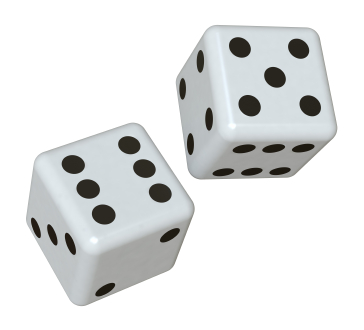
\includegraphics[height=.32\textwidth]{../images/dados.jpg}} & \quad\quad &
  {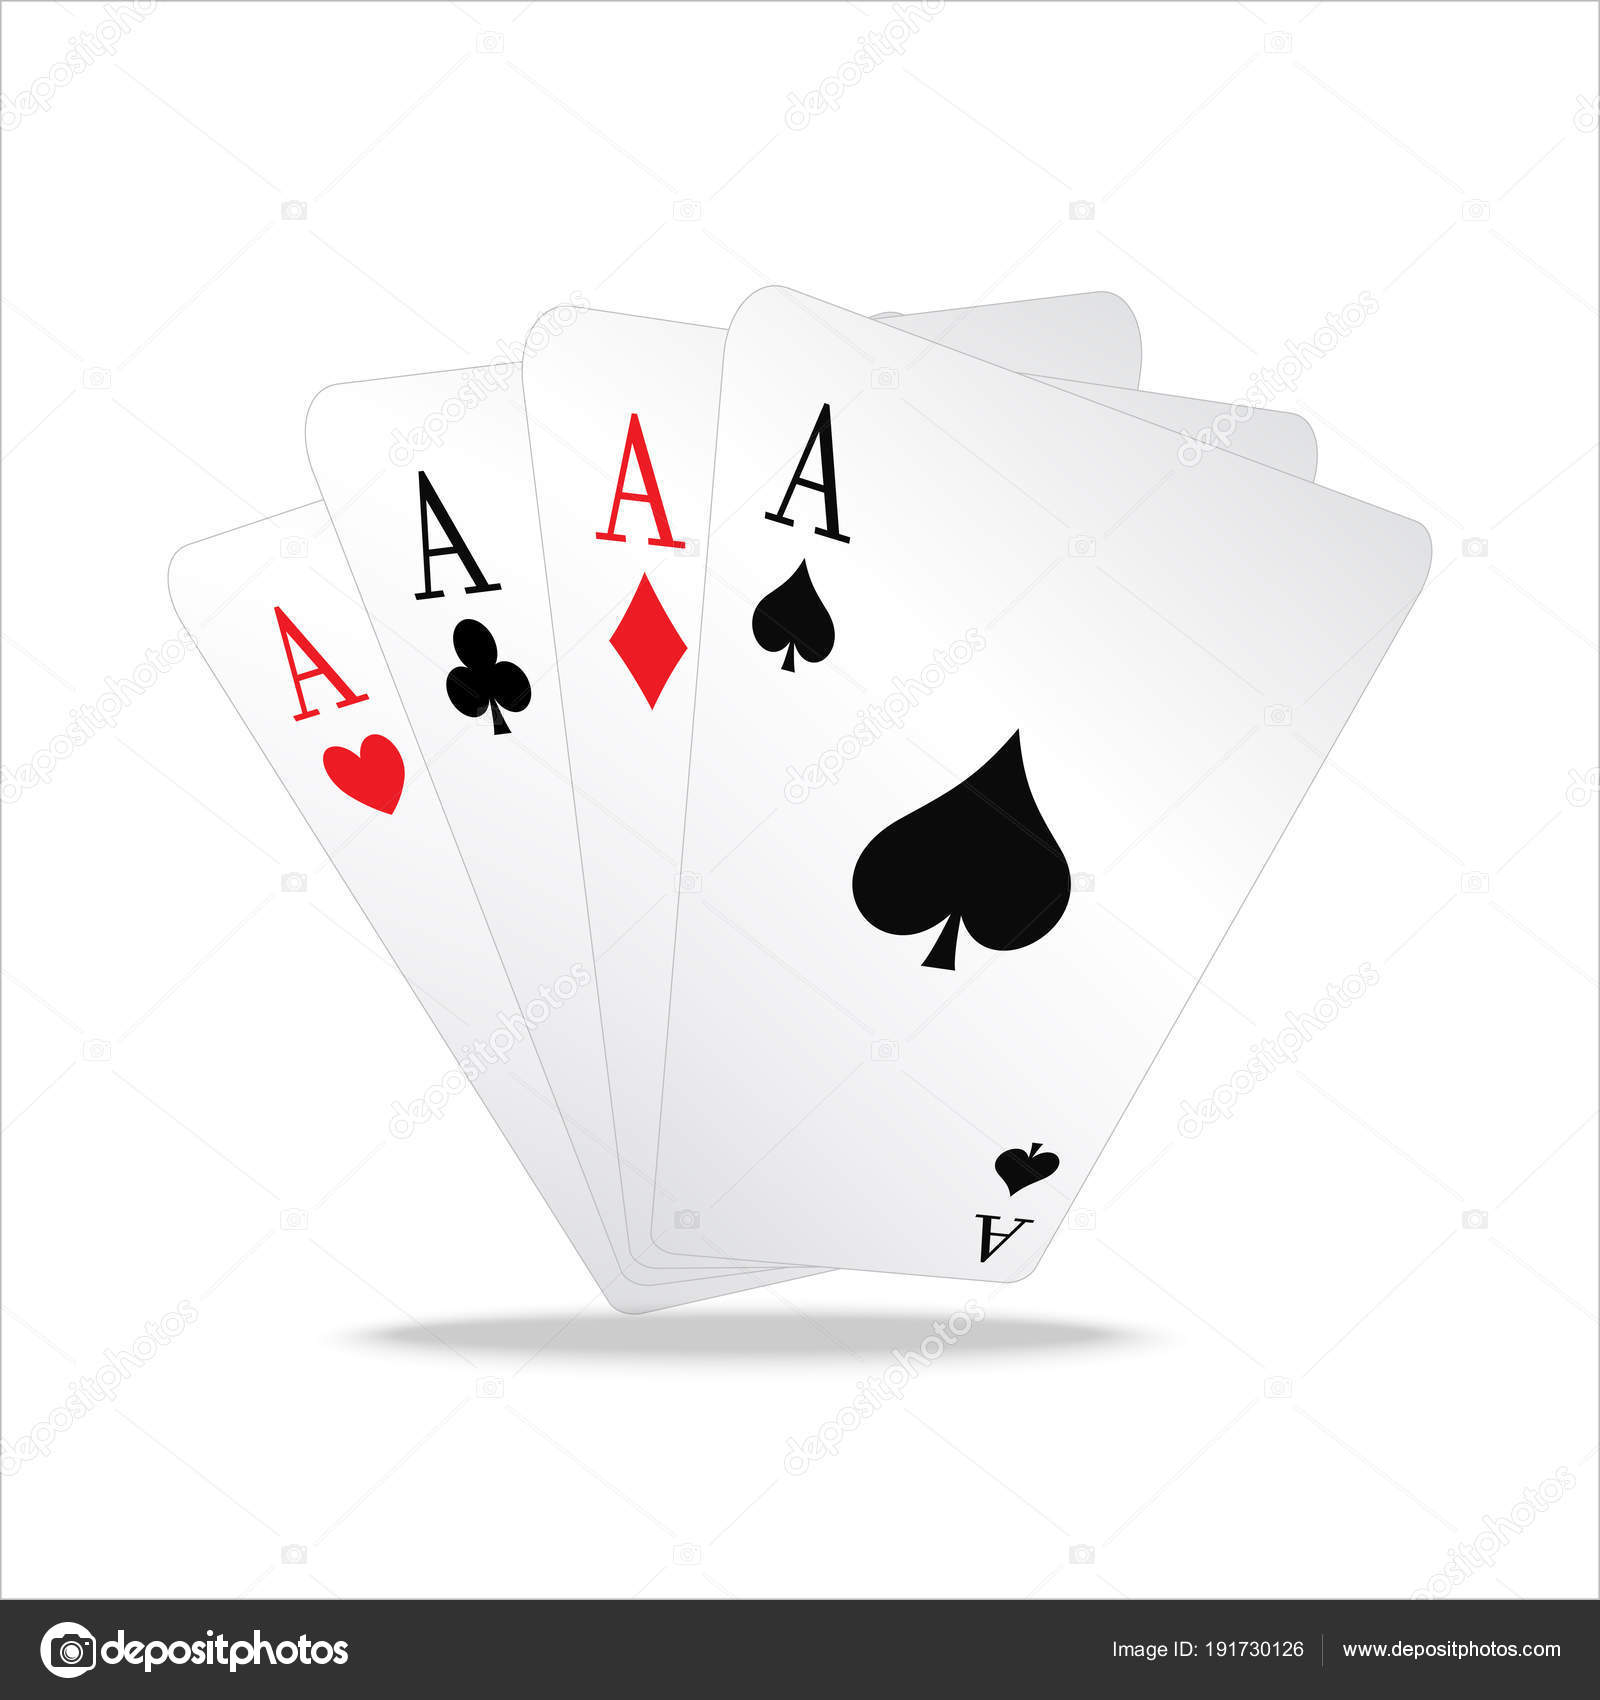
\includegraphics[height=.32\textwidth]{../images/cartas.jpg}}
}
\end{tabular}
\end{center}

\column{.45\textwidth}
\begin{block}{Informaci\'on incompleta}
\onslide<3>{
Informaci\'on parcial sobre algunas de las acciones que fueron tomadas previamente.
}
\end{block}
\begin{center}
\begin{tabular}{@{}ccccc@{}}
  \visible<3->{{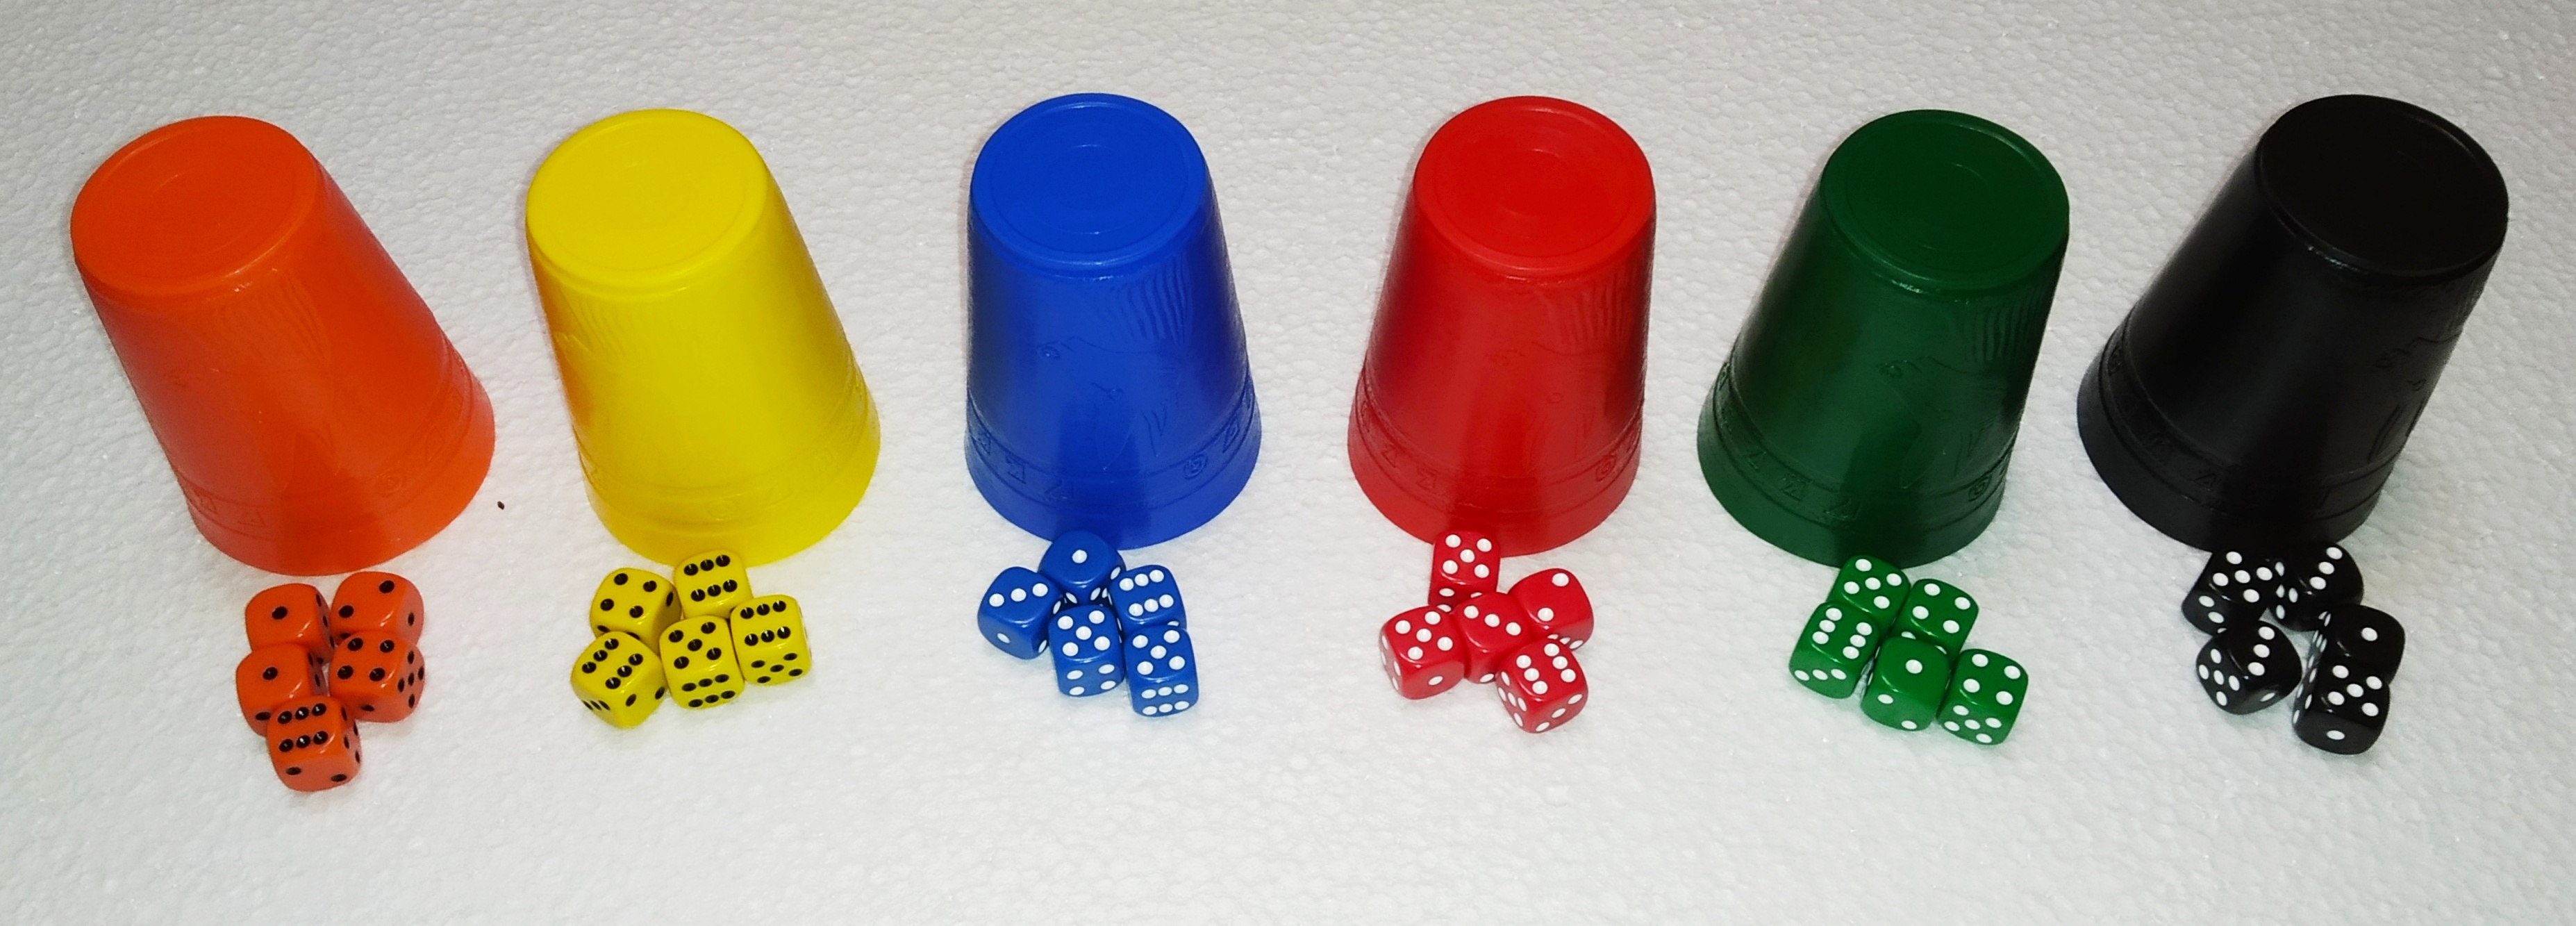
\includegraphics[height=.32\textwidth]{../images/dudo.jpg}}}
\end{tabular}
\end{center}
\end{columns}

\vspace{.5cm}
\visible<4->{\Alert{Interrogantes}}
\begin{itemize}
  \item \visible<5->{?`Qu\'e significa que un juego sea resuelto?}
  \item \visible<6->{?`Cu\'ando un jugador juega de forma \'optima?}
\end{itemize}
\end{frame}

\begin{frame}{\Large Objetivo General}%\Large Objetivos}
%\begin{block}{Objetivo General}
\centering{Comprender los conceptos en el \'area de juegos de dos personas que involucran informaci\'on incompleta y no determinismo, as\'i como implementar los algoritmos para resolverlos, realizando experimentos sobre distintos juegos que son capturados por el modelo.}
%\end{block}
% \begin{itemize}
%   \visible<2->{\onslide<2>{\item Comprender los diferentes modelos de juegos.}}
%   \visible<3->{\onslide<3>{\item Comprender diferentes conceptos de soluci\'on.}}
%   \visible<4->{\onslide<4>{\item Comprender los resultados te\'oricos m\'as relevantes.}}
%   \visible<5->{\onslide<5>{\item Implementar los algoritmos de Regret Matching y Counterfactual Regret Minimization.}}
%   \visible<6->{\onslide<6>{\item Implementar clases que permitan representar los juegos.}}
%   \visible<7->{\onslide<7>{\item Realizar experimentos sobre los juegos propuestos.}}
%   \visible<8->{\onslide<8>{\item Evaluar las estrategias obtenidas.}}
% \end{itemize}
\end{frame}

\begin{frame}{\Large Juegos en Forma Normal o Estrat\'egica}

\Alert{Piedra, papel o tijera}
\vspace{.5cm}

\begin{tabular}{l |c | c | c | l }
\multicolumn{1}{c}{} &  \multicolumn{1}{c}{ $\mathcal{R}$ \raisebox{3pt}{\tikzmark{sp2}}(piedra)} & \multicolumn{1}{c}{$\mathcal{P}$ (papel)} & \multicolumn{1}{c}{$\mathcal{S}$ (ti\raisebox{3pt}{\tikzmark{ep2}}jera)} & \ \
\visible<3>{\textcolor{blue!70!black}{jugador 2}} \\ \cline{2-4}
$\mathcal{R}$ (piedra) & $0,0$ & $-1,1$ & $1,-1$ & \\ \cline{2-4}
$\mathcal{P}$ (p\raisebox{3pt}{\tikzmark{p1}}apel)  & $1,-1$ & $0,0$ & $-1,1$ & \\ \cline{2-4}
$\mathcal{S}$ (tijera) & $-1,1$ & $1,$\raisebox{3pt}{\tikzmark{u}}$-1$ & $0,0$ & \\ \cline{2-4}
\multicolumn{1}{c}{} &
  \multicolumn{3}{c}{
    \only<4>{\small{primer jugador \textbf{gana} 1}}
    \only<5>{\small{segundo jugador \textbf{pierde} 1}}
  }
 & \multicolumn{1}{c}{}\\
\multicolumn{2}{l}{\visible<2>{\textcolor{blue!70!black}{jugador 1}}} &
\multicolumn{3}{c}{}
\end{tabular}

\vspace{.5cm}
\begin{columns}[t]
\column{.45\textwidth}
\visible<6->{
\Alert{Elementos}
\begin{enumerate}
  \onslide<7, 13->{\item Jugadores.}
  \onslide<8, 13->{\item Acciones o estrategias puras: $\mathcal{R}$, $\mathcal{P}$, $\mathcal{S}$.}
  \onslide<9, 13->{\item Funci\'on de pago o utilidades.}
\end{enumerate}
}
\column{.52\textwidth}
\visible<10->{
\Alert{Estrategias}
\begin{enumerate}
  \onslide<11, 13->{\item Estrategias puras: siempre se elige la misma acci\'on.}
  \onslide<12, 13->{\item Estrategias mixtas: cada acci\'on se elige con cierta probabilidad.}
\end{enumerate}
}
\end{columns}

\visible<2>{
\begin{tikzpicture}[remember picture,overlay]
\coordinate[draw,line width=.75pt,blue!70!black,ellipse, inner xsep=22pt, inner ysep=24pt, fit={(pic cs:p1)}] {};
\end{tikzpicture}
}
\visible<3>{
\begin{tikzpicture}[remember picture,overlay]
\coordinate[draw,line width=.75pt,blue!70!black,ellipse,inner ysep=7pt,fit={(pic cs:sp2) (pic cs:ep2)}] {};
\end{tikzpicture}
}
\visible<4-5>{
\begin{tikzpicture}[remember picture,overlay]
\coordinate[draw,line width=.75pt,blue!70!black,ellipse,inner xsep=15, inner ysep=5pt,fit={(pic cs:u)}] {};
\end{tikzpicture}
}
\end{frame}

\begin{frame}{\Large Juegos en Forma Normal o Estrat\'egica}

\Alert{Batalla de los sexos}
\vspace{.5cm}

\begin{columns}
\column{.7\textwidth}
\begin{tabular}{ c c | c | c |}

& \multicolumn{1}{c}{} & \multicolumn{2}{c}{\AlertSecondary{Jos\'e}} \\
& \multicolumn{1}{c}{} &
\multicolumn{1}{c}{\quad\ ballet \quad\quad} &
\multicolumn{1}{c}{\quad\,b\'eisbol \quad\quad}  \\ \cline{3-4}

\multirow{2}{*}{\AlertSecondary{Mar\'ia}}
& ballet    &
  \onslide<2->{\ \ \onslide<2-13, 15->{$2$}\onslide<2-12, 15->{$,\,$}\mymark{ballet}\onslide<2-12, 14->{$1$} \mymark{elegirBallet}&
  \onslide<2-12, 15->{$0,\,$}\mymark{differentsA}\onslide<2-12, 14->{$0$} \\ \cline{3-4}}
& b\'eisbol &
  \onslide<2->{\onslide<2-13, 15->{$0$}\onslide<2-12, 15->{$,\,$\mymark{differentsB}$0$} &
  \onslide<2-12, 15->{$1$\mymark{beisbol}$,2$} \\ \cline{3-4}}

\end{tabular}
\ellipse{3}{12pt}{5pt}{differentsA}
\ellipse{3}{12pt}{5pt}{differentsB}
\ellipse{4,10,12-15}{12pt}{5pt}{ballet}
\ellipse{5,12,15}{12pt}{5pt}{beisbol}
\ellipse{9}{2.5cm}{7pt}{elegirBallet}

\column{.3\textwidth}
\only<3-5>{
\begin{itemize}
  \item
    \only<3>{Ninguno obtiene ganancia.}
    \only<4>{Mar\'ia obtiene una ganancia mayor que Jos\'e.}
    \only<5>{Jos\'e obtiene una ganancia mayor que Mar\'ia.}
\end{itemize}
}

\only<13-14>{
  \begin{itemize}
    \item
      \only<13>{Mar\'ia no tiene motivos para cambiar su estrategia.}
      \only<14>{Jos\'e no tiene motivos para cambiar su estrategia.}
  \end{itemize}
}

\only<9-10>{
  \begin{itemize}
  \item
    \only<9>{Si Mar\'ia siempre elige ballet.}
    \only<10>{Lo mejor para Jos\'e es siempre elegir ballet.}
  \end{itemize}
}

\only<17->{
  {Lanzar una moneda
  \begin{enumerate}
  \item cara $\implies$ ballet
  \item sello $\implies$ b\'eisbol
  \end{enumerate}}
}
\end{columns}

\vspace{.5cm}

\begin{columns}
\column{.4\textwidth}
\visible<6->{
\Alert{Conceptos}
\begin{enumerate}
  \onslide<7>{\item Ganancia Esperada}
  \onslide<8-10>{\item Mejor Respuesta}
  \onslide<11-15>{\item Equilibrio de Nash}
  \onslide<16->{\item Equilibrio Correlacionado}
\end{enumerate}

\column{.5\textwidth}

\only<7>{Valor promedio que un determinado jugador obtendr\'ia si jugara infinitas veces y cada jugador utiliza una estrategia dada.}
\only<8-10>{La mejor forma en que puede jugar un jugador dadas las estrategias seleccionadas de sus oponentes.}
\only<11-15>{Cada jugador utiliza una mejor respuesta frente a las estrategias de sus oponentes.}
\only<16->{Puede haber cooperaci\'on entre los jugadores.}
}
\end{columns}
\end{frame}

\begin{frame}{\Large Equilibrio de Nash}

\Alert{Piedra, papel o tijera}
\vspace{.5cm}

\begin{tabular}{l |c | c | c | }
\multicolumn{1}{c}{} &  \multicolumn{1}{c}{ $\mathcal{R}$ (piedra)} & \multicolumn{1}{c}{$\mathcal{P}$ (papel)} & \multicolumn{1}{c}{$\mathcal{S}$ (tijera)} \\ \cline{2-4}
$\mathcal{R}$ (piedra) &
  \onslide<1-2,5,8->{\ 0}\onslide<1-2,8->{,\ 0} &
  \onslide<1-3,8->{-1}\mymark{rp}\onslide<1-2,8->{,\ 1} &
  \onslide<1-2,7->{\ 1}\onslide<1-2,8->{,-1} \\ \cline{2-4}
$\mathcal{P}$ (papel)  &
  \onslide<1-2,5,8->{\ 1}\onslide<1-2,8->{,}\mymark{pr}\onslide<1-2,6,8->{-1} &
  \onslide<1-3,8->{\ 0}\onslide<1-2,8->{,}\onslide<1-2,6,8->{\ 0} &
  \onslide<1-2,7->{-1}\mymark{ps}\onslide<1-2,8->{,}\onslide<1-2,6,8->{\ 1} \\ \cline{2-4}
$\mathcal{S}$ (tijera) &
  \onslide<1-2,5,8->{-1}\mymark{sr}\onslide<1-2,8->{,}\onslide<1-2,4,8->{\ 1} &
  \onslide<1-3,8->{\ 1}\onslide<1-2,8->{,}\onslide<1-2,4,8->{\mymark{sp}-1} &
  \onslide<1-2,7->{\ 0}\onslide<1-2,8>{,}\onslide<1-2,4,8->{\ 0} \\ \cline{2-4}
\end{tabular}

\ellipse{2-3}{15pt}{5pt}{rp}
\ellipse{4}{15pt}{5pt}{sp}
\ellipse{5}{15pt}{5pt}{sr}
\ellipse{6}{15pt}{5pt}{pr}
\ellipse{7}{15pt}{5pt}{ps}

\vspace{.75cm}
\visible<8->{\RedAlert{No todos los juegos tienen un equilibrio de Nash en estrategias puras.}}

\visible<9->{
  \vspace{.5cm}
  \begin{block}{Teorema de Nash}
  Todo juego finito tiene al menos un equilibrio de Nash (en estrategias mixtas).
  \end{block}
}
\end{frame}

\begin{frame}{Juegos de Dos Jugadores de Suma Cero}

\visible<2->{\Alert{Observaciones previas}}
\begin{itemize}
  \visible<3->{\item En el juego \textbf{batalla de los sexos} los equilibrios de Nash no son soluciones satisfactorias.}
  \visible<4->{\item Diferentes equilibrios de Nash llevan a diferentes ganancias esperadas.}
\end{itemize}

\vspace{.5cm}
\visible<5->{\Alert{Equilibrio de Nash en Juegos de Dos Jugadores de Suma Cero}}
\begin{enumerate}
  \visible<6->{\item Soluci\'on satisfactoria.}
  \visible<7->{\item Valor del juego $u$: ganancia esperada del primer jugador cuando ambos jugadores utilizan \textbf{cualquier} equilibrio de Nash.}
  \visible<8->{\item El primer jugador puede garantizar una ganancia esperada de \textbf{al menos} $u$ independientemente de la estrategia de su oponente.}
  \visible<9->{\item El segundo jugador puded garantizar una ganancia esperada de \textbf{al menos} $-u$ independientemente de la estrategia de su oponente.}
\end{enumerate}

\end{frame}

\begin{frame}{\Large Regret Matching}

\Alert{Algoritmos para calcular un Equilibrio de Nash}
\begin{itemize}
  \item Juegos de dos jugadores de suma cero.
\end{itemize}
\begin{enumerate}
  \onslide<2->{\item Se juega de forma repetida a trav\'es del tiempo $t = 1, 2, 3, ...$.}
  \onslide<3->{\item A tiempo $t+1$ cada jugador elige una acci\'on siguiente una estrategia mixta determinada.}
  \onslide<4->{\item La \textbf{estrategia emp\'irica} converge a un equilibrio de Nash.}
\end{enumerate}
\vspace{.25cm}
\visible<5->{
\Alert{?`C\'omo calcular la distribuci\'on de probabilidad?}
\begin{itemize}
  \item Diferentes formas de calcular la distribuci\'on de probabilidad conducen a diferentes algoritmos.
\end{itemize}
}
\vspace{.25cm}
\visible<6->{
\begin{block}{Regret}
M\'etrica de \bold<7->{arrepentimiento} de no haber elegido una acci\'on en particular.
\end{block}
}
\end{frame}

\begin{frame}{\Large Regret Matching}
\begin{block}{Regret}
M\'etrica de \textbf{arrepentimiento} de no haber elegido una acci\'on en particular.
\end{block}
\vspace{.6cm}
\begin{columns}
\column{.45\textwidth}
\Alert{Tres procedimientos}
\begin{enumerate}
  \onslide<3-5,10->{\item Regret condicional.}
  \onslide<6,10->{\item Vector invariante de probabilidad de la matriz\\de regret condicional.}
  \onslide<7->{\item Regret incondicional.}
\end{enumerate}

\column{.5\textwidth}
\visible<2->{%
\begin{tabular}{|p{9mm}p{9mm}p{9mm}|p{5mm}|}
\hline
$\mathcal{R}, \mathcal{S}$ & $\mathcal{R}, \mathcal{P}$ & $\mathcal{S}, \mathcal{S}$ & $\bar{u}$\\ \hline
1 & -1 & 0 & 0\\ \hline
\end{tabular}
}

\vspace{.3cm}
\visible<4-5,8->{%
\begin{tabular}{|p{9mm}p{9mm}p{9mm}|p{5mm}|}
\hline
  $\AlertSecondary{\mathcal{\only<4,8>S\only<5,9->P}}, \mathcal{S}$ &
  $\AlertSecondary{\mathcal{\only<4,8>S\only<5,9->P}}, \mathcal{P}$ &
  $\only<4-5>{\mathcal{S}}\AlertSecondary{\only<8>{\mathcal{S}}\only<9->{\mathcal{P}}}, \mathcal{S}$ &
  $\bar{u}$\\ \hline
  \only<4,8>0\only<5,9->{-1}&\only<4,8>1\only<5,9->0&\only<4-5,8>0\only<9->{-1}&\only<5,9->-$\frac{\only<4-5,8>1\only<9->2}{3}$\\ \hline
\end{tabular}
}
\vspace{.3cm}
\visible<4-5, 8->{
\begin{tabular}{p{50mm}}
 \only<4>{$R_1(\mathcal{R}, \mathcal{S}\,) = \frac{1}{3} - 0 = \frac{1}{3}$}
 \only<5>{$R_1(\mathcal{R}, \mathcal{P}) = -\frac{1}{3} - 0 = -\frac{1}{3}$}
 \only<8>{$R_1(\mathcal{S}) =  \frac{1}{3} - 0 =  \frac{1}{3}$}
 \only<9->{$R_1(\mathcal{P}) = -\frac{2}{3} - 0 = -\frac{2}{3}$}
\end{tabular}
}
\end{columns}
\end{frame}

\begin{frame}{\Large Regret Matching}
\Alert{Observaciones}
\begin{enumerate}
  \visible<2->{\item Las probabilidades son elegidas proporcional a los regrets positivos.}
  \visible<3->{\item El regret va a cero cuando el n\'umero de juegos va a infinito.}
  \visible<4->{\item Supongamos que el regret incondicional de cualquier acci\'on es menor que $\varepsilon > 0$.}
  \begin{itemize}
    \visible<5->{\item La estrategia emp\'irica es una aproximaci\'on a un equilibrio de Nash que se encuentra una distancia no mayor que $\varepsilon$.}
    \visible<6->{\item $\varepsilon$-equilibrio de Nash.}
  \end{itemize}
\end{enumerate}
\end{frame}

\begin{frame}{\Large Resultados Experimentales}
\vspace{.5cm}
\begin{columns}[t]
\column{.45\textwidth}
\Alert{Evaluaci\'on y Correctitud}
\begin{enumerate}
  \onslide<2,15->{\visible<2->{\item Gr\'aficas del regret incondicional con respecto al n\'umero de iteraciones.}}
  \onslide<3,15->{\visible<3->{\item Problema equivalente de programaci\'on lineal.}}
  \visible<4->{\item Explotabilidad\only<14->{: $\varepsilon = \varepsilon_1 + \varepsilon_2$}.}
\end{enumerate}
\column{.5\textwidth}
\visible<5->{%
\Alert{\only<5-8>{Equilibrio de Nash $\sigma^* = (\sigma^*_1, \sigma^*_2)$}\only<9->{Aproximaci\'on $\sigma' = (\sigma'_1, \sigma'_2)$}}
\visible<6-8, 10->{%
\begin{itemize}
  \onslide<6,10-11,15->{\visible<6-8, 10->{\item Primer jugador garantiza una ganancia esperada de al menos \only<6-8>{$u$}\only<10->{$u-\varepsilon_1$}.}}
  \onslide<7-8, 12-13,15->{\visible<7-8, 12->{\item Segundo jugador garantiza una ganancia esperada de \only<7>{al menos $-u$.}\only<8, 12->{a lo sumo} \only<8>{$u$}\only<12->{$u+\varepsilon_2$} \only<8, 12->{para el primer jugador.}}}
\end{itemize}}
}
\end{columns}
\begin{center}
  \begin{tikzpicture}
  \visible<5->{\draw[<->, very thick] (-5.25, 0) -- (5.25, 0);}
  \visible<5->{\draw[dashed] (0, 1.5) -- (0, -1.5);}
  \visible<5->{\node[align=center] at (0.15, 0.2) {\small{$u$}};}
  \visible<5->{\draw[fill=black] (0, 0) circle (0.05cm);}
  \visible<6>{\draw[->, rounded corners, blue, very thick](0, 0) -- (0, -0.6) -- (5.25, -0.6);}
  \visible<6->{\draw[->, rounded corners, blue, very thin](0, 0) -- (0, -0.6) -- (5.25, -0.6);}
  \visible<6->{\node[text width=3.5cm] at (3.5,-1) {$u_1(\sigma_1^*, \sigma_2) \geq u $};}
  \only<7>{\node[text width=3.5cm] at (-3,-1) {$u_2(\sigma_1, \sigma^*_2) \geq -u $};}
  \visible<7->{\draw[->, rounded corners, red, very thin](0, 0) -- (0, -0.5) -- (-5.25, -0.5);}
  \visible<7-8>{\draw[->, rounded corners, red,  very thick](0, 0) -- (0, -0.5) -- (-5.25, -0.5);}
  \visible<8->{\node[text width=3.5cm] at (-3,-1) {$u_1(\sigma_1, \sigma^*_2) \leq u $};}
  \visible<10->{\draw[<->](-0.01, 1) -- (-1.5, 1);}
  \visible<10->{\draw[dashed] (-1.5, 2) -- (-1.5, -0.45);}
  \visible<10->{\node[text width=1cm] at (-0.4, 1.25) {$\varepsilon_1$};}
  \visible<10->{\node[align=left] at (-0.9, 0.2) {\small{$u-\varepsilon_1$}};}
  \visible<10->{\draw[fill=black] (-1.5, 0) circle (0.05cm);}
  \visible<11->{\draw[->, rounded corners, blue, very thin](-1.5, 0) -- (-1.5, 0.6) -- (5.25, 0.6);}
  \visible<11>{\draw[->, rounded corners, blue, very thick](-1.5, 0) -- (-1.5, 0.6) -- ( 5.25, 0.6);}
  \visible<11->{\node[text width=3.5cm] at (3.5, 1) {$u_1(\sigma'_1, \sigma_2) \geq u - \varepsilon_1$};}
  \visible<12->{\draw[<->](0.01, 1) -- (0.8, 1);}
  \visible<12->{\draw[dashed] (0.8, 2) -- (0.8, -0.45);}
  \visible<12->{\node[text width=1cm] at (0.7, 1.25) {$\varepsilon_2$};}
  \visible<12->{\node[align=left] at (1.35, 0.2) {\small{$u+\varepsilon_2$}};}
  \visible<12->{\draw[fill=black] (0.8, 0) circle (0.05cm);}
  \visible<13->{\draw[->, rounded corners, red, very thin](0.8, 0) -- (0.8, 0.5) -- (-5.25, 0.5);}
  \visible<13>{\draw[->, rounded corners, red,  very thick]( 0.8, 0) -- ( 0.8, 0.5) -- (-5.25, 0.5);}
  \visible<13->{\node[text width=3.5cm] at (-3.25, 1) {$u_1(\sigma_1, \sigma'_2) \leq u + \varepsilon_2$};}
  \visible<14->{\draw[<->](-1.5, 1.7) -- (0.8, 1.7);}
  \visible<14->{\node[text width=1cm] at (0.1, 2) {$\varepsilon$};}
  \end{tikzpicture}
\end{center}
\end{frame}
\end{document}
